\section{Auroral Emissions}\label{sec:physicsemissions}

Given the historical record of deep red aurora observable at latitudes at least as low as $10^\circ$ \citep{silverman2008}, many nations and cultures have experienced aurora at least once a generation.
A rule of thumb for naked-eye visible aurora is the energy flux must be at least $\unit[1]{mW\, m^{-2}}$ or a volume emission rate greater than \unit[1]{kR}.
Modern semiconductor-based photoelectron-multiplying imaging chips give wide dynamic range and industry-leading single-photoelectron sensitivity, revealing detailed auroral features at intensities far below what human eyes and emulsified film can accomplish at high frame rates.
Purple aurora thought to correspond to \unit[427.8]{nm} and \unit[391.4]{nm} emissions is occasionally seen at the lower edge of auroral displays, when the viewing geometry and conditions are such that it is not overwhelmed by the far more intense \unit[557.7]{nm} and \unit[630.0]{nm} emissions.
%TODO This paper has info on cross sections
%\url{https://www.nist.gov/sites/default/files/documents/srd/jpcrd387.pdf}

The notional auroral spectrum in Figure~\ref{fig:VJaurora} shown over the wavelength span of interest is for a bright ICB III aurora.
\begin{figure}
	\includegraphics[width=\textwidth,trim=5 10 5 1,clip]{gfx/AuroralSpectrumLogVJ}
	\caption{Auroral spectrum in wavelength range of interest, from \citet{vallancejones1974}. }\label{fig:VJaurora}
\end{figure}
To reject metastable emissions with lifetime $\tau \gg\unit[1]{ms}$ that would smear out prompt auroral emissions, the DMC and HiST systems observed through Schott BG3 bandstop filters with specified performance in Figure~\ref{fig:BG3trans}. 
\begin{figure}\centering
	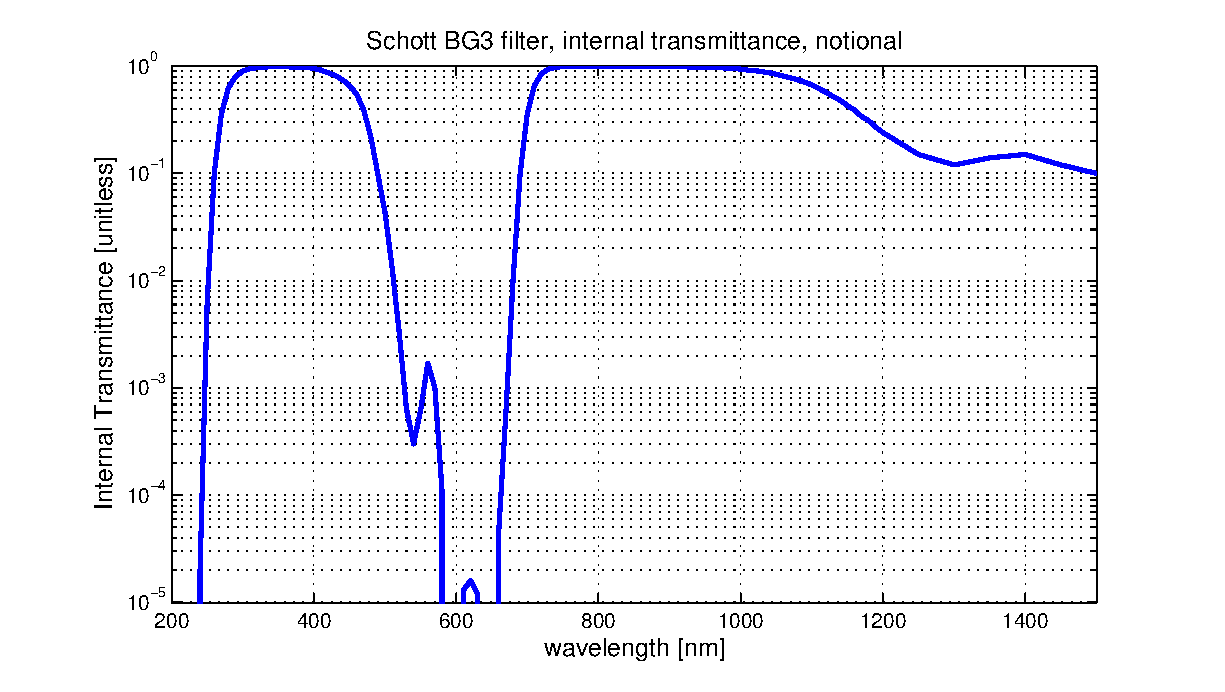
\includegraphics[width=\textwidth]{gfx/BG3transLog}
	\caption{Schott BG3 filter response}\label{fig:BG3trans}
\end{figure}
A comparison of the BG3 filter with historical and contemporary prompt emissions filters is given in Figure~\ref{fig:filters}.
The deep notch in the BG3 spectral response rejects most intense long-lifetime emissions. 
The notional EMCCD window transmission and Quantum Efficiency (QE) are shown in Figure~\ref{fig:EMCCDwindQE}.
\begin{figure}\centering
	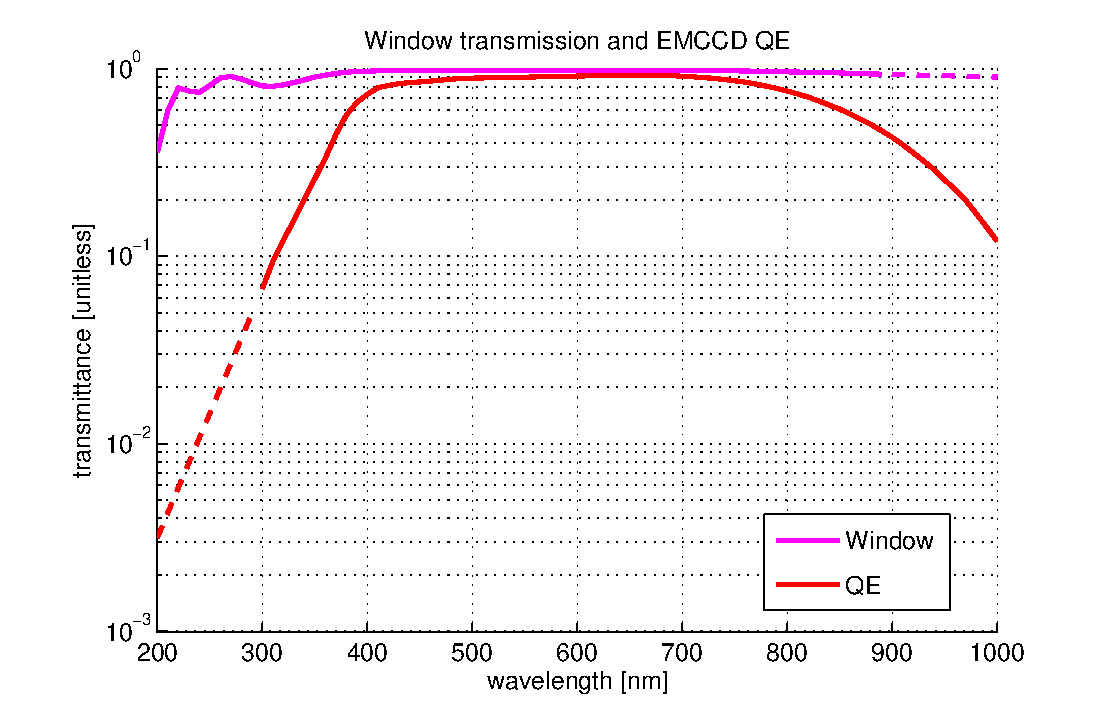
\includegraphics[width=\textwidth]{gfx/EMCCDwindowQELog}
	\caption{EMCCD window transmission and QE (extrapolated values dashed)}\label{fig:EMCCDwindQE}
\end{figure}  
The notional total system response in the wavelength range $\lambda \in [200,1000]$ nm is shown in Figure~\ref{fig:systemSpectralResp}.
\begin{figure}\centering
	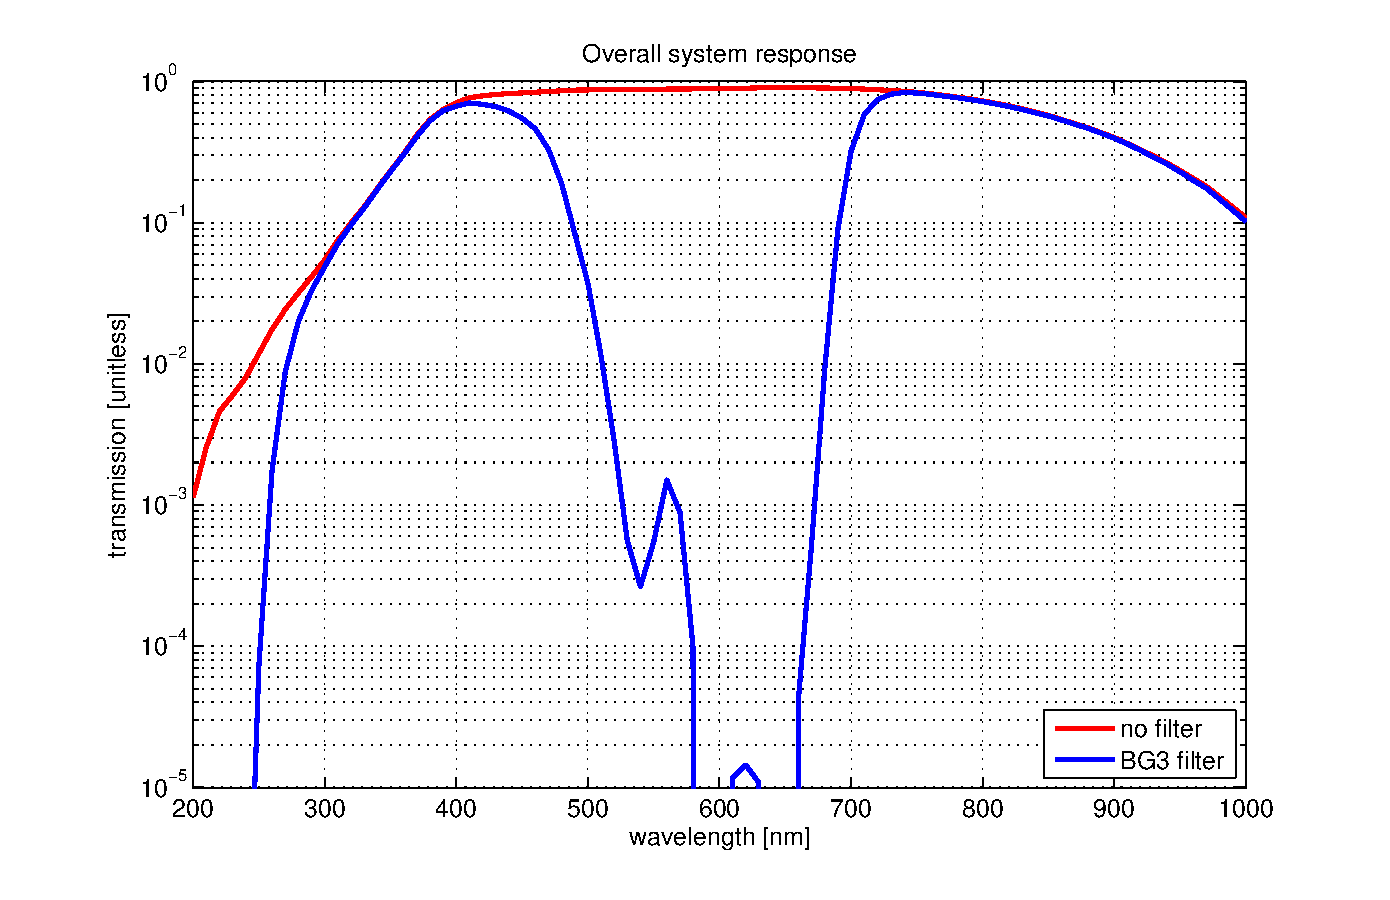
\includegraphics[width=\textwidth]{gfx/EMCCDoverallTlog}
	\caption{Overall optical transmission from lens through EMCCD chip}\label{fig:systemSpectralResp}
\end{figure}
The overall HiST transmission including atmospheric absorption, particularly significant at UV is shown in Figure~\ref{fig:optTrans}.
Several well-known auroral emission lines are given in Table~\ref{tab:spectrum} along with the optical system attenuation noted in Figure~\ref{fig:auroragen}. 

Brightness observed for the \unit[427.8]{nm} line, often taken as a proxy for high-energy precipitation has been given in the \unit[0.1..3]{kR} range \citep{dashkevich2006}.
% below 150km, dissociative recombination becomes important
Typical parameters for auroral flux as given by \citet{sandholtbook} are in Table~\ref{tab:typaurora}.
\begin{table}\centering
	\caption{Notional auroral emissions characteristics~\citep{sandholtbook}.}
    \label{tab:typaurora}
	\begin{tabular}{clll}
        \toprule
		wavelength [nm] & state & excitation energy [eV] & peak alt. [km] \\
		\midrule
		630.0 & [O] ($^1$D) & $\sim5.6$ & 200 \\
		557.7 & [O] ($^1$S) & $\sim10$ & 120 \\
		427.8 & N2$^+$ 1N & $\sim 100$ & 100 \\
        \bottomrule
	\end{tabular}
\end{table}
A starting point for the notional particle flux is typically of order $\unit[10^{13}]{m^{-2}s^{-1}}$ with energy flux of order $\unit[10]{mW \,m^{-2}}$.
A classic technique for estimating characteristic intensity $E_0$ looking up the magnetic zenith flux tube is based on the intensity ratio of line spectra.
From \citet{rees1974}, the typical ratio of $I_{6300}/I_{4278}$ is about 0.05..15, for $I_{6300}/I_{5577}$ the typical ratio is about 0.03..2.
However, for structured aurora these ratioing techniques fall apart (become highly inaccurate) since they completely lose validity away from magnetic zenith. 
%TODO justify this assertion!
An auroral observation system capable of observing within several degrees of magnetic zenith is necessary to quantify the differential number flux $\Phi_{top}$ driving structured aurora.
HiST is the first such system capable of estimating auroral precipitation characteristics with \unit[20]{ms} cadence, a rate compatible with the fastest ISR measurements as described in chapter~\ref{chapter:fusion}.

	
